%%%%%MISE EN PAGE%%%%%%%
    

\documentclass[10pt,a4paper]{article}
\usepackage[utf8]{inputenc}
\usepackage[T1]{fontenc}
\usepackage[french]{babel}
\usepackage{multicol}
\usepackage[left=2cm, right=2cm, bottom=1.85cm, top=1.5cm]{geometry}

\usepackage{fancyhdr}
\usepackage{multicol}
\pagestyle{fancy}

%\renewcommand{\headrulewidth}{1pt}
%\fancyhead[C]{\textbf{page \thepage}} 
\fancyhead[R]{Seconde 1}

\renewcommand{\footrulewidth}{1pt}
\fancyfoot[C]{\textbf{page \thepage}} 
\fancyfoot[L]{Lycée Jacques Brel}
\fancyfoot[R]{Année 2022-2023}


%\newcommand{\TDoc}[1]{
%\begin{center}
%{\setlength{\fboxsep}{10pt}  % Ecart texte-boite
%\shadowbox{\textbf{\Large{#1}}}}
%\end{center}
%\vspace{1.5cm}}
    
 \usepackage{fancybox}   %pour l'encadré du titre shadowbox
 \usepackage{stmaryrd}   %pour utiliser correctement les crochets pour les ensembles de définitions
 \usepackage[normalem]{ulem}
 \usepackage{graphicx}
 %\usepackage{wrapfig} %texte coulé autour d'une image
 \usepackage{soul} % souligné
 \usepackage{nonfloat}
%MATHEMATIQUES
\usepackage{amsmath,amsfonts} 
\usepackage{tikz}
\newcommand{\N}{\mathbb{N}}
\newcommand{\Z}{\mathbb{Z}}
\newcommand{\D}{\mathbb{D}}
\newcommand{\Q}{\mathbb{Q}}
\newcommand{\R}{\mathbb{R}}
\newcommand{\C}{\mathbb{C}}
\newcommand{\K}{\mathbb{K}}
\newcommand{\F}{\mathbb{F}}


\newtheorem{de}{Définition} % les définitions et les théorèmes sont
\newtheorem{theo}{Théorème}    % numérotés par section
\newtheorem{prop}[theo]{Proposition} 
\newtheorem{pro}[theo]{Propriété} 
\newtheorem{exe}{Exemple} 
\newtheorem{exo}{Exercice}  
\newtheorem{qe}{Question de cours}
%%%%%%%%%%%%
\makeatletter
\newlength{\longA}
\newlength{\longB}
\newenvironment{BoiteShadow}[3][\linewidth]{%
\addtolength{\longA}{#2}
\addtolength{\longB}{#3}
\begin{Sbox}\begin{minipage}{#1}}%
{\end{minipage}\end{Sbox}%
\setlength{\fboxsep}{\longA}
\setlength{\shadowsize}{\longB}
\shadowbox{\unhbox\@Sbox}\par}
\makeatother
%%%%%%%

\title{}

%%%%%%%%%%%%%%%%
\begin{document}

\begin{BoiteShadow}{10pt}{8pt}
\Huge{Feuille d'exercice $n^{\circ}1$: Ensembles de nombres}
 \end{BoiteShadow}
%\section{Connaissance du cours}
%Vous avez cinq minutes pour répondre aux questions suivantes. \textbf{Dans votre cahier}, répondre aux questions suivantes \textbf{sans regarder le cours}. Si vous n'arrivez pas à répondre au bout des cinq minutes, répondez aux question en allant voir le cours. 

%\begin{enumerate}
%\item Je connais l'ensemble des nombres entiers naturels, des nombres entiers relatifs, des nombres décimaux et des nombres rationnels? Les décrire.  
%\item Comment sont caractérisés les nombres décimaux? 
%\item Comment additionner et multiplier des nombres rationnels?
%\item Comment multiplier ou diviser par une puissance de $10$?	
%\end{enumerate}

\section{Ensembles de nombres}

\begin{exo}
    Parmi les cinq ensembles vus en cours, dire quel est le plus petit qui contient chacun des nombres suivants :
    \begin{enumerate}
        \item $-345$
        \item $2,0756$
        \item $78$
        \item $\frac{5}{9}$
        \item $\frac{235}{5}$
        \item $2\pi$
        \item $\sqrt{36}$
        \item $\frac{2,97}{0,01}$
        \item $-5 \times 10^{-2}$
        \item $24,63 \times 10$
    \end{enumerate}
\end{exo}

\begin{exo}
  Ecrire les nombres décimaux suivants sous forme d'une fraction de la forme 
  $\cfrac{a}{10^{n}}$. Où $a\in\Z$ et $n\in\N$.
  \begin{enumerate}
    \item $a=3,3967$
    \item $b=0,0031415235$
    \item $c=25,75$
    \item $d=0,2192$
  \end{enumerate}
\end{exo}

\begin{exo}
  Montrer que les nombres suivants sont décimaux, puis donner une écriture sous la forme 
  $\cfrac{a}{10^{n}}$. Où $a\in\Z$ et $n\in\N$.
  \begin{enumerate}
    \item $a=\cfrac{9}{20}$
    \item $b=\cfrac{7}{50}$
    \item $c=\cfrac{13}{4}$
    \item $d=\cfrac{17}{5}$
  \end{enumerate}
\end{exo}

\begin{exo}
  Ecrire les nombres suivants sous forme décimale.
  \begin{enumerate}
    \item $a=\cfrac{11}{20}$
    \item $b=5+\cfrac{3}{10}+\cfrac{9}{100}+\cfrac{2}{1000}$
    \item $c=\cfrac{2}{100}-\cfrac{5}{10}$
    \item $d=\cfrac{-7}{40}$
  \end{enumerate}
\end{exo}

\begin{exo}
Le nombre $4,156$ peut s'écrire sous la forme: $4,156=4+\cfrac{1}{10}+\cfrac{5}{100}+\cfrac{6}{1000}$. Faire de même avec les nombres suivants:
\begin{enumerate}
\item $A=5,432$.
\item $B=0,45$
\item $C=0,867$
\item $D=-7,1324$	
\end{enumerate}
	
\end{exo}

\newpage

\begin{exo}
.
\begin{enumerate}
\item Donner la valeur décimale des fractions suivantes: $\cfrac{1}{2}$; $\cfrac{1}{4}$; $\cfrac{1}{5}$; $\cfrac{1}{8}$ et $\cfrac{1}{10}$.
\item En déduire la valeur décimale des fractions suivantes:
 $\cfrac{5}{2}$; $\cfrac{3}{5}$; $\cfrac{7}{10}$; $\cfrac{7}{4}$ et $\cfrac{9}{5}$. 
 \item Donner la valeur décimale de: $\cfrac{7}{80}$ et $\cfrac{9}{32}$. 	
\end{enumerate}
	
\end{exo}

\begin{exo}
Mettre les fractions suivantes au même dénominateur: $\cfrac{1}{2}$; $\cfrac{1}{3}$; $\cfrac{1}{4}$ et $\cfrac{1}{5}$. 	En déduire la valeur de $\cfrac{1}{2}+\cfrac{1}{3}+\cfrac{1}{4}+\cfrac{1}{5}$.
\end{exo}


\begin{exo}
Calculer les expressions suivantes et donner le résultat sous la forme d'une fraction irréductible.
\begin{multicols}{5}\noindent
$$A= \cfrac{-72}{5}+\cfrac{96}{35}\times\cfrac{-5}{12}\quad$$
\columnbreak
$$B = \cfrac{\cfrac{-8}{3}-6}{\cfrac{-2}{3}+4}\quad$$
\columnbreak
$$ C= \frac{-1}{2}\div\left(\frac{3}{2}+\frac{13}{7}\right)\quad$$
\columnbreak
$$D= \cfrac{\cfrac{8}{3}+10}{\cfrac{-1}{8}+10} $$
\columnbreak
$$E= \cfrac{7}{4}\div\left(\cfrac{-9}{10}+\cfrac{-4}{7}\right)$$
\end{multicols}

\end{exo}
	
\begin{exo}
Ecrire $10^{n}$ pour $n\in\{-5;-4;-3;-2;-1;0;1;2;3;4;5\}$. On rappelle que si $n\in\N$ on a $10^{-n}=\frac{1}{10^{n}}$. 	
\end{exo}


\begin{exo}
    Complétez les pointillés par un des symboles $\in$, $\notin$, $\subset$, $\not\subset$
    \begin{multicols}{3}
        \begin{enumerate}
            \item $-4\;\ldots\;\mathbb{N}$
            \item $3\;\ldots\;\mathbb{Z}$
            \item $\mathbb{N}\;\ldots\;\mathbb{Z}$
            \item $\mathbb{D}\;\ldots\;\mathbb{Z}$
            \item $\frac{3}{16}\;\ldots\;\mathbb{D}$
            \item $\frac{16}{3}\;\ldots\;\mathbb{D}$
            
        \end{enumerate}
    \end{multicols}
    \end{exo}

\newpage

\setcounter{exo}{11}


\begin{exo}
    \begin{enumerate}
        \item Exprimer sous la forme d'intervalle, d'inégalité et de représentation graphique l'ensemble des nombres $x$ qui vérifient $\lvert x \rvert \leq 3$
        \item Généraliser en exprimant d'une de ces trois manières l'ensemble des $x$ qui vérifient $\lvert x \rvert \leq \ell$ pour un nombre réel $\ell > 0$ donné.
        \item En utilisant la définition de la distance entre deux nombres, Exprimer l'ensemble des nombres qui sont à une distance de moins de $\ell$ du nombre $a$  pour $a \in \R$ et $\ell \in \R^+$
    \end{enumerate}

    
\end{exo}

\begin{exo}
  Placez les nombres décimaux suivants sur la droite des réels, en utilisant l'échelle 1 unité = 8 centimètres, puis écrivez les nombres dans l'ordre croissant séparés par des $<$ :
  $$\frac{7}{20}; 0,5; 0,03145; \frac{39}{40}$$
\end{exo}

\begin{exo}
  On donne des nombres réels. Donner un encadrement des nombres entre deux 
  décimaux à $10^{-2} = 0{,}01$ près. Puis donner le résultats sous forme d'un intervalle d'amplitude $10^{-2}$.
  Exemple: $\pi=3{,}1415235......$ alors $3,14<\pi<3,15\Longleftrightarrow 
  \pi\in]3{,}14;3{,}15[$.
 \begin{enumerate}
   \item $a=\sqrt{3}$
   \item $b=-\frac{\pi}{5}$
   \item $c=53{,}2109$
   \item $d=\frac{8}{7}$
 \end{enumerate}
\end{exo}

\begin{exo}
  Donner traduire les encadrements ou les inégalités suivants sous forme 
  d'intervalles. 
  Exemples:  ou 
  
  \begin{enumerate}
  \item Exemple 1 : $-2,56<x\leq 4,7\Longleftrightarrow x\in ]-2,56;4,7]$
  \item Exemple 2 : $x\geq 7\Longleftrightarrow x\in[7;+\infty[$.
    \item $-2\leq x<-1,6 $
    \item $x\leq -7,2$
    \item $-1\leq a\leq 1$
    \item $-7,56<y$
    \item $-9,29<z\leq 9$
  \end{enumerate}
\end{exo}

\begin{exo}
  Représenter graphiquement chaque intervalle suivant sur une droite réelle.
  \begin{enumerate}
      \item $[3;6]$
      \item $[-2;4[$
      \item $]-\infty;5]$
  \end{enumerate}
\end{exo}

\begin{exo}
  Pour chaque description des intervalles A et B, dire si les ensembles $A \cap B$ et $A \cup B$ sont des intervalles et si oui, écrire cet intervalle.
  \begin{enumerate}
      \item $A=[1;4]$ et $B=[2;6]$
      \item $A=[2;5]$ et $B=[-2;8]$
      \item $A=[1;2]$ et $B=[3;4]$
  \end{enumerate}
\end{exo}

\begin{exo}
    Recopiez et complétez le tableau suivant en faisant correspondre intervalle, inégalités, et représentation graphique
    \begin{center}
    \renewcommand{\arraystretch}{2}
    \begin{tabular}{|c|c|c|}
    \hline
    Intervalle	& C'est l'ensemble des réels $x$ tels que &	Représentation graphique sur la droite des réels\\
    \hline
    $]-2 ; 6[$ &  & \\
    \hline
     & $x < 7$ & \\
    \hline
     &  & \begin{tikzpicture}[>=latex]
    \draw[->] (0,0) --(6,0);
    \draw[blue, line width = 3pt] (2,0) --(5,0);
    \node[blue, line width = 3pt] at (5,0) {$\Big[$};
    \node[blue, line width = 3pt] at (2,0) {$\Big[$};
    \node[below=8pt] at (5,0) {$5$};
    \node[below=8pt] at (2,0) {$2$};
    %\foreach \xp in {2.2,2.4,...,4.8}{\node[] at (\xp,0) {/};}
\end{tikzpicture}\\
    \hline
    $[16 ; +\infty[$ & & \\
    \hline 
    & $6 \leq x \leq 8$  & \\
    \hline
    \end{tabular}
    \end{center}
\end{exo}
\setcounter{chapter}{3}
\newpage

\setcounter{section}{2}
\setcounter{exo}{0}
\section{Vecteurs}

\subsection{Dans un repère}


\begin{exo}
    Dans la figure ci-contre, représenter : \begin{enumerate}
        \item Dessiner le vecteur $\overrightarrow{AB}$
        \item Placer le point D, image de C par la translation de vecteur $\overrightarrow{AB}$
        \item Placer le point E, image de C par la translation de vecteur $\overrightarrow{BA}$
        \item Placer le point F, image de B par la translation de vecteur $\overrightarrow{AC}$
        \item Placer le point G, image de C par la translation de vecteur $\overrightarrow{AC}$
        \item Placer le point H, image de A par la translation de vecteur $\overrightarrow{u}$
        
    \end{enumerate}
    \center
    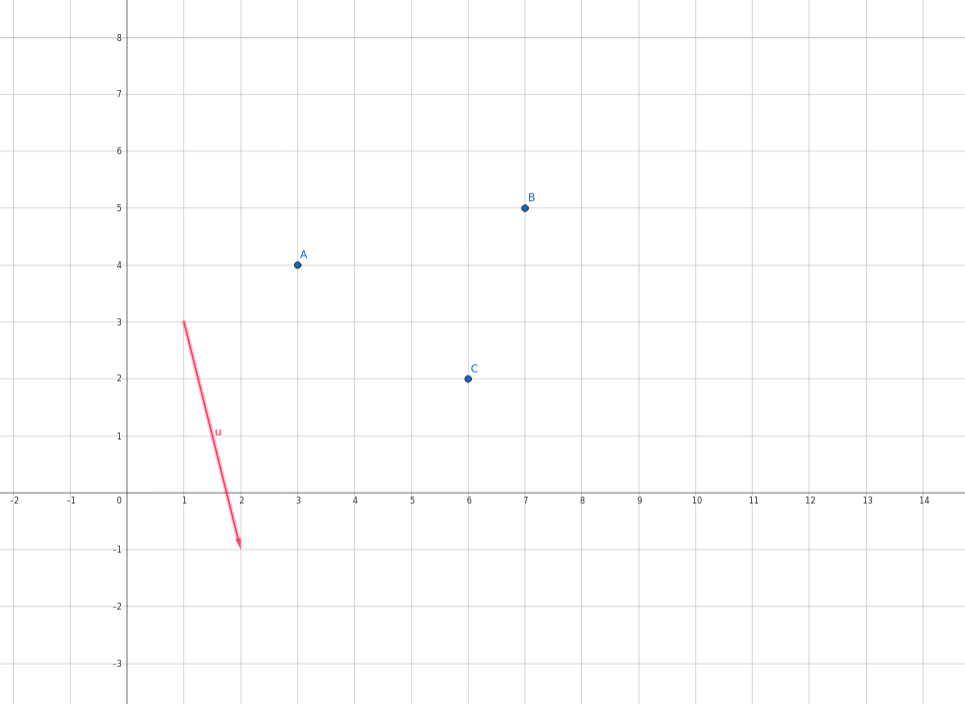
\includegraphics[width=0.7\textwidth]{assets/Exo1-vecteurs.png} 

\end{exo}

\begin{exo}
    \begin{enumerate}
        \item Sur une droite réelle que vous dessinerez, où 1 carreau représente 1 unité, placez les nombres $A=-2$, $B=4$ et $C=1$.
        \item Placez sur la droite le nombre $D$ qui est l'image de $C$ par la translation de vecteur $\overrightarrow{AB}$.
        \item Que vaut D? Que peut-on dire de la distance $CD$?
        \item Félicitations, vous savez calculer l'image d'un vecteur en 1 dimension. Le faire en 2 dimensions consistera juste à mener le même raisonnement sur l'abscisse puis l'ordonnée de points, qui auront deux coordonnées au lieu d'en avoir une. Ceci n'est pas une question, relisez juste les 2 premiers paragraphes du cours sur les vecteurs.
    \end{enumerate}
\end{exo}

\begin{exo}
    \begin{enumerate}
        \item Dessinez un repère orthonormé
        \item Placez les points $A$ de coordonnées $(1,5)$ et le point $B$ de coordonnées $(3,2)$.
        \item Dessinez le vecteur $\overrightarrow{AB}$. Quelles sont les coordonnées de ce vecteur?
    \end{enumerate}
\end{exo}

\newcommand*{\Coord}[2]{% 
  \ensuremath{ 
    \begin{pmatrix} 
      #1\\ 
      #2 
    \end{pmatrix}}}


\begin{exo}
    Soient les points $A(0,1)$, $B(2,3)$, $C(2,1)$, $D(-2,0)$, $E(3,0)$. Calculer les coordonnées des vecteurs
    \begin{multicols}{3}
        \begin{enumerate}
            \item $\overrightarrow{AB}$
            \item $\overrightarrow{BA}$
            \item $\overrightarrow{BC}$
            \item $\overrightarrow{AC}$
            \item $\overrightarrow{CD}$
            \item $\overrightarrow{AD}$
            \item $\overrightarrow{DE}$
            \item $\overrightarrow{AE}$
            \item $\overrightarrow{EA}$
        \end{enumerate}
    \end{multicols}
\end{exo}

\begin{exo}
    Sur un repère orthonormé que vous tracerez, placer :
    \begin{enumerate}
            \item Le point $A(1,1)$ et son image $A'$ par la translation de vecteur de coordonnées $\Coord{2}{4}$
            \item Le point $B(-1,1)$ et son image $B'$ par la translation de vecteur de coordonnées  $\Coord{-3}{2}$
            \item Le point $C(-1,2)$ et son image $C'$ par la translation de vecteur de coordonnées  $\Coord{2}{-1}$
            \item Le point $D(-2,-2)$ et son image $D'$ par la translation de vecteur de coordonnées  $\Coord{0}{-4}$
            \item Le point $E(4,2)$ et son image $E'$ par la translation de vecteur $\overrightarrow{0}$
    \end{enumerate}
\end{exo}

\begin{exo}
    Dans chacun des cas suivants, donner les coordonnées du point $C'$, image de $C$ par la translation de vecteur $\overrightarrow{AB}$ :
    \begin{enumerate}
        \item $A$ a pour coordonnées $(2,1)$, $B$ a pour coordonnées $(3,4)$ et $C$ a pour coordonnées $(1,1)$
        \item $A$ a pour coordonnées $(5,2)$, $B$ a pour coordonnées $(3,3)$ et $C$ a pour coordonnées $(2,1)$
        \item $A$ a pour coordonnées $(-1,2)$, $B$ a pour coordonnées $(3,0)$ et $C$ a pour coordonnées $(6,4)$
        \item $A$ a pour coordonnées $(6,8)$, $B$ a pour coordonnées $(1,2)$ et $C$ a pour coordonnées $(0,3)$
        \item $A$ a pour coordonnées $(\frac{3}{2},\frac{1}{3})$, $B$ a pour coordonnées $(\frac{1}{2},\frac{7}{3})$ et $C$ a pour coordonnées $(1,1)$
        \item $A$ a pour coordonnées $(\frac{1}{2},2)$, $B$ a pour coordonnées $(\frac{1}{3},\frac{7}{2})$ et $C$ a pour coordonnées $(0,\frac{1}{3})$
        \item $A$ a pour coordonnées $(\sqrt{2},\pi)$, $B$ a pour coordonnées $(2,\frac{2}{7})$ et $C$ a pour coordonnées $(1,1)$
    \end{enumerate}
\end{exo}


\begin{exo}
    Sur chacun des dessins suivants, construire le vecteur $\overrightarrow{AC}$ tel que $\overrightarrow{AC}=\overrightarrow{u}+\overrightarrow{v}$
\end{exo}
\begin{tabular}{|c|c|c|}
    \hline
    \begin{minipage}{0.3\textwidth}
        \includegraphics[width=\textwidth]{assets/Cap1.PNG} 
    \end{minipage} & 
    \begin{minipage}{0.3\textwidth}
        \includegraphics[width=\textwidth]{assets/Cap2.PNG} 
    \end{minipage} & \begin{minipage}{0.3\textwidth}
        \includegraphics[width=\textwidth]{assets/Cap3.PNG} 
    \end{minipage}\\
    \hline
\end{tabular}

\begin{exo}
    \begin{enumerate}
        \item Soient $\overrightarrow{u}$ le vecteur de coordonnées $\Coord{-6}{8}$ et $\overrightarrow{v}$ de coordonnées $\Coord{4}{5}$. Quelles sont les coordonnées de $\overrightarrow{u}+\overrightarrow{v}$ ?
        \item On pose des points $A$,$B$,$C$ et $D$ de coordonnées $A(4,2)$, $B(-2,3)$, $C(-4,-1)$ et $D(2,0)$. Donnez les coordonnées des vecteurs 
        \begin{multicols}{3}
            \begin{enumerate}
                \item $\overrightarrow{AB}$
                \item $\overrightarrow{CD}$
                \item $\overrightarrow{AB}+\overrightarrow{CD}$
                \item $-\overrightarrow{AB}$
                \item $\overrightarrow{DC}$
                \item $\overrightarrow{BA}+\overrightarrow{DC}$
                \item $\overrightarrow{DC}+\overrightarrow{AB}$
                \item $2 \times \overrightarrow{AB}$
                \item $-2 \times \overrightarrow{AB}$
            \end{enumerate}
        \end{multicols}
    \end{enumerate}
\end{exo}

\begin{exo}
    Recopiez et complétez les égalités suivantes en utilisant la relation de Chasles :
    \begin{multicols}{2}
        \begin{enumerate}
            \item $\overrightarrow{AC} + \overrightarrow{CE} = \dots$
            \item $\overrightarrow{AD} + \overrightarrow{\dots E} = \overrightarrow{AE}$
            \item $\overrightarrow{D\dots} + \overrightarrow{BC} = \overrightarrow{DC}$
            \item $\overrightarrow{\dots K} + \overrightarrow{KL} = \overrightarrow{PL}$
            \item $\overrightarrow{AC} + \overrightarrow{CF} + \overrightarrow{FG} = \dots$
            \item $\overrightarrow{MB} + \overrightarrow{CM} = \dots$
            \item $\overrightarrow{DG} + \overrightarrow{GD} = \dots$
            \item $\overrightarrow{AB} - \overrightarrow{AB} = \dots$
        \end{enumerate}
        
    \end{multicols}
\end{exo}

\begin{exo}[Démonstration de la relation de Chasles]
    Soient $A(x_A,y_A)$, $B(x_B,y_B)$, $C(x_C,y_C)$.  Déterminez les coordonnées de $\overrightarrow{AB}$,$\overrightarrow{BC}$ et $\overrightarrow{AC}$.  En déduire que $\overrightarrow{AB}+\overrightarrow{BC}=\overrightarrow{AC}$
\end{exo}

\newpage


\begin{minipage}{0.35\textwidth}
    \begin{exo}
        \begin{enumerate}
            \item         Dans le dessin ci-contre, donnez toutes les relations de colinéarité existant entre les vecteurs.
            \item Parmi les vecteurs qui sont colinéaires, lesquels ont le même sens?
            \item Soient u,v et w des vecteurs non nuls tels que u est colinéaire à v, et v colinéaire à w. Montrer que u est colinéaire à w. On pourra revenir à la définition de la colinéarité du cours.
        \end{enumerate}
    \end{exo}
\end{minipage}
\begin{minipage}{0.62\textwidth}
    \center
    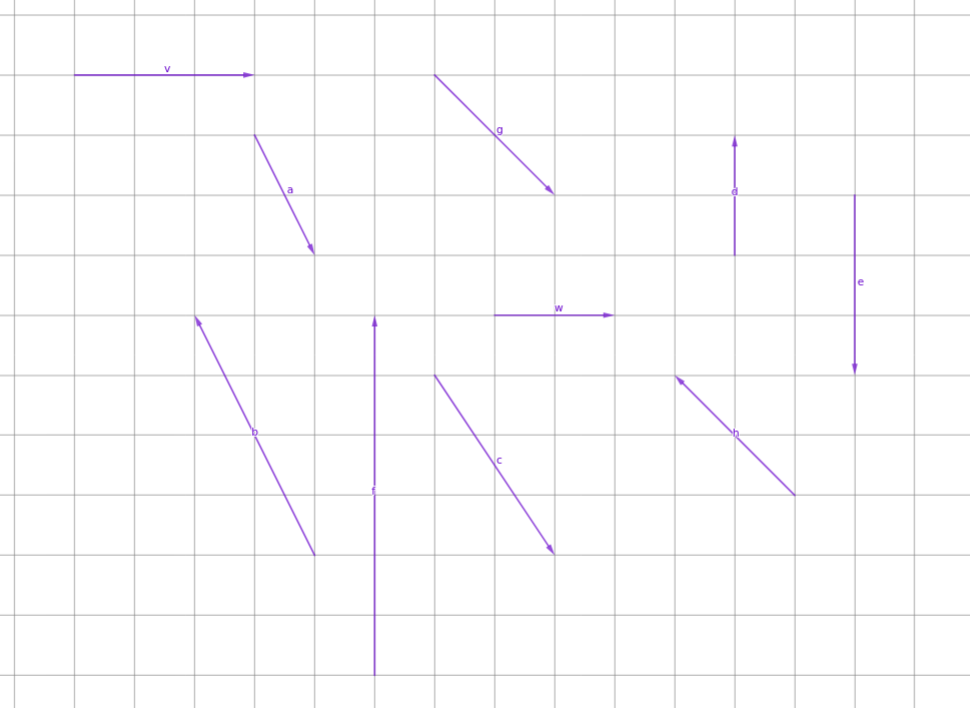
\includegraphics[width=0.95\textwidth]{assets/ExoColineaires-Vecteurs.png}
\end{minipage}

\begin{exo}
    Parmi les vecteurs suivants dont on donne les coordonnées, faites des groupes de vecteurs colinéaires, en justifiant votre classement. : 
    \begin{multicols}{3}
        \begin{enumerate}
            \item  $\overrightarrow{a} \Coord{-1}{2}$
            \item  $\overrightarrow{b} \Coord{1}{1}$
            \item  $\overrightarrow{c} \Coord{3}{-6}$
            \item  $\overrightarrow{d} \Coord{-5}{-5}$
            \item  $\overrightarrow{e} \Coord{3}{2}$
            \item  $\overrightarrow{f} \Coord{2}{1}$
            \item  $\overrightarrow{g} \Coord{-2}{0}$
            \item  $\overrightarrow{h} \Coord{4}{2}$
            \item  $\overrightarrow{i} \Coord{1}{0}$
        \end{enumerate}
    \end{multicols}
\end{exo}

\begin{exo}
    On va ici démontrer une propriété du cours à l'aide de propriétés vues les années précédentes sur les parallélogrammes.
    
    Soient $A,B,C$ et $D$ quatre points tels que $\overrightarrow{AB}$=$\overrightarrow{CD}$.
    
    \begin{enumerate}
        \item faites un dessin, représentant A,B,C et D qui vérifient la condition de l'énoncé.
        \item Montrez que les longueurs des segments $[AB]$ et $[CD]$ sont égales.
        \item En utilisant la relation de Chasles, montrez que $\overrightarrow{AC}=\overrightarrow{BD}$. En déduire une relation entre les longueurs des segments $[AC]$ et $[BD]$.  (Pour la première partie de la question, on pourra décomposer le vecteur $\overrightarrow{AD}$ de deux manières différentes)
        \item Rappelez les différentes manières de montrer qu'un quadrilatère est un parallélogramme
        \item Démontrez, en utilisant une des méthodes de la réponse précédente, que ABDC est un parallélogramme.
    \end{enumerate}
    
\end{exo}



\newpage

\section{Trucs plus balaises pour plus tard}


Celui ci nécessite les équations cartésiennes de droites.
\begin{exo}
    Le but de cet exercice est de démontrer le théorème du cours qui fait le lien entre colinéarité de vecteurs et alignements de points ou parallélisme de droites. Soient des points $A$,$B$ deux points distincts du plan et un vecteur $\overrightarrow{u}$ non nul.
    \begin{enumerate}
        \item Montrez que s'il existe un point $C$ du plan et deux réels $k$ et $k'$ tel que $\overrightarrow{AC}=k\overrightarrow{u}$ et $\overrightarrow{AC}=k'\overrightarrow{u}$, alors $\overrightarrow{AB}$ est colinéaire à $\overrightarrow{u}$.  (On posera les coordonnées des points et des vecteurs définis, et on appliquera la définition de la colinéarité). Puis donnez l'équation d'une droite qui contient les points $A, B$ et $C$.
        \item On suppose maintenant que des points $E$ et $F$ sont tels que $\overrightarrow{EF}$ et $\overrightarrow{u}$ ne sont pas colinéaires. On pose $E'$ l'image de $E$ par la translation de vecteur $\overrightarrow{u}$ et $F'$ l'image de $F$ par la même translation.  Montrez que les droites $(EE')$ et $(FF')$ sont parallèles 
    \end{enumerate}
\end{exo}

La même sur le parallélogramme : non pour celui là j'ai besoin juste des distances et de Chasles...

\end{document}